\section{Theorie}
\label{sec:Theorie}

Die Elementarladungen kann man durch den sogenannten Millikan-Versuch bestimmen. Dazu müssen kleine Öltröpfchen 
in das vertikale Feld eines Plattenkondensators gebracht werden. Durch Reibung erhalten diese eine elektrische Ladung und folglich 
erfahren sie eine Kraft bedingt durch das E-Feld. Auf das Tröpfchen wirken dann insgesamt 4 Kräfte, welche in \autoref{fig:Kräfte} schematisch dargestellt sind.
\begin{figure}
    \centering
    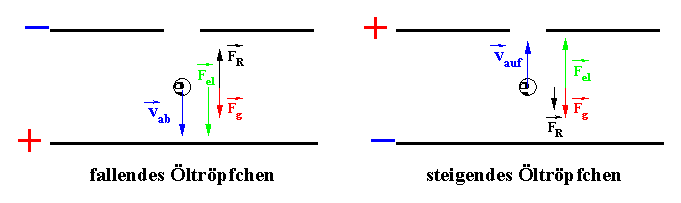
\includegraphics{Kräfte.pdf}
    \caption{Darstellung der auf das Öltröpfchen wirkende Kräfte \cite{ap503}.}
    \label{fig:Kräfte}
\end{figure}
Die einzelnen Kräfte werden durch folgende Formeln beschrieben
\begin{align*}
    \vec{F_{\text{g}}} &=m\vec{g}\quad (\text{Gewichtskraft}),\\
    \vec{F_{\text{R}}} &=6\pi r \eta_{\text{L}} \vec{v}\quad (\text{Reibungskraft}),\\
    \vec{F_{\text{el}}}&=q\cdot \vec{E}\quad (\text{Kraft durch das E-Feld}) ,\\
    \vec{F_{\text{a}}} &=m_{\text{L}}\cdot g\quad (\symup{Auftriebskraft}).
\end{align*}
Hierbei ist $m$ die Masse des Tröpfchens, $\vec{g}$ die Erdbeschleunigung, $r$ der Radius des Tröpfchens, $\eta_{\text{L}}$ die Viskosität der Luft,
$\vec{v}$ die Geschwindigkeit, $q$ die Ladung, $E$ das E-Feld des Plattenkondensators und $m_{\text{L}}$ die Masse der durch das Tröpfchen verdrängten Luft.
Bei ausgeschaltetem E-Feld kann dann, wenn die Gleichgewichtsgeschwindigkeit des Tröpfchens $\vec{v_0}$ erreicht ist ein Kräftegleichgewicht aufgestellt werden
\begin{align*}
    \vec{F_{\text{g}}}-\vec{F_{\text{a}}}&= \vec{F_{\text{R}}}\. ,\\
    \frac{4\pi}{3}r^3(\rho_{\text{Öl}}-\rho_{\text{L}})g&= 6\pi r \eta_{\text{L}} \vec{v}\. .
\end{align*} 
Nach Umstellen folgt so Für den Radius des Tröpfchen
\begin{equation*}
r=\sqrt{\frac{9\eta_{\text{L}}v_0}{2g(\rho_{\text{Öl}}-\rho_{\text{L}})}}
\end{equation*}
Wenn nun eine Spannung angelegt wird, steigt oder sinkt das Tröpfchen. Für die Richtung spielt die Polung des Kondensators eine große Rolle (siehe \autoref{fig:Kräfte}).
Wirkt die elektrische Kraft nach unten, erhöht sich die Sinkgeschwindigkeit und die Kräfte Gleichung erweitert sich zu
\begin{equation*}
    \frac{4 \pi}{3} r^3\left(\rho_{Öl}-\rho_L\right) g-6 \pi \eta_L r v_{ab}=-q E\. .
\end{equation*}
Wenn das Tröpfchen steigt, ergibt sich die Kräftegleichung zu
\begin{equation*}
    \frac{4 \pi}{3} r^3\left(\rho_{Öl}+\rho_L\right) g+6 \pi \eta_L r v_{auf}=+q E\. .
\end{equation*}
Aus diesen beiden Gleichungen lässt sich nun die Ladung des Tröpfchens über die Formel 
\begin{equation*}
    q=3 \pi \eta_L \sqrt{\frac{9}{4} \frac{\eta_L}{g} \frac{\left(v_{a b}-v_{a u f}\right)}{\left(\rho_{O e l}-\rho_L\right)}} \cdot \frac{\left(v_{a b}+v_{a u f}\right)}{E}
\end{equation*}
und der Tröpfchenradius 
\begin{equation*}
    \sqrt{\frac{9}{2} \frac{\eta_L}{g} \frac{\left(v_{a b}-v_{a u f}\right)}{\left(\rho_{O e l}-\rho_L\right)}}
\end{equation*}
bestimmt werden.
Da die Tröpfchen kleiner sind als die mittlere freie Weglänge in Luft $\vec{l}$, muss die Viskosität $\eta_{\text{L}}$ der Luft über die Gleichung
\begin{equation*}
    \eta_{\text{eff}}=\eta_{\text{L}}\left(\frac{1}{1+A\frac{1}{r}}\right)=\eta_{\text{L}}\left(\frac{1}{1+B\frac{1}{pr}}\right)
\end{equation*}
ermittelt werden. Die Größe $B=6.17\cdot 10^{-3} \text{ Torr}\cdot \unit{\cm}$ ist der Cunningham-Korrekturterm.
Da die mittlere freie Weglänge $\vec{l}$ umgekehrt proportional zum Luftdruck $p$ ist, ist die korrigierte Ladung
\begin{equation*}
    q^{\frac{2}{3}}_{korrigiert}= q^{\frac{2}{3}}_0\left(1+B\frac{1}{pr}\right)\. .
\end{equation*}